% Anhang
%

\chapter{Profiling}

For the profiling an own implementation is used based on wall clock timings.
The iteration loop \ref{ConnectAlg} is instrumented. An own implementation is
chosen to have full control about the disk and memory access of the profiler.
So io interruptions caused by the profiler are avoided.

Used code to get current timestamp:

\begin{lstlisting}
enum
{
	MICROSEC = (timeunit_t)1,
	MILLISEC = MICROSEC * 1000,
	SECONDS  = MILLISEC * 1000,
};

uint64_t get_timestamp ()
{
    struct timeval now;
    gettimeofday (&now, (struct timezone*)0);
    return  (uint64_t) now.tv_usec + 
            (uint64_t) now.tv_sec * SECONDS;
}
\end{lstlisting}


The measured timings are written to an csv file, which has e.g. the following content:
\begin{lstlisting}
0;0;run;0;3793;116429658;
0;0;loadSynapses;0;2622330;4432049;
0;0;sort;0;4519751;5770458;
0;0;communicate;0;5770465;6366961;
\end{lstlisting}
Each row specifies one measurement the columns contain the rank number, thread number, function name,
iteration number, start time and finish time respectively.

To get an overview the numbers are plotted in a raster plot.

\begin{figure}[ht!]
\centering
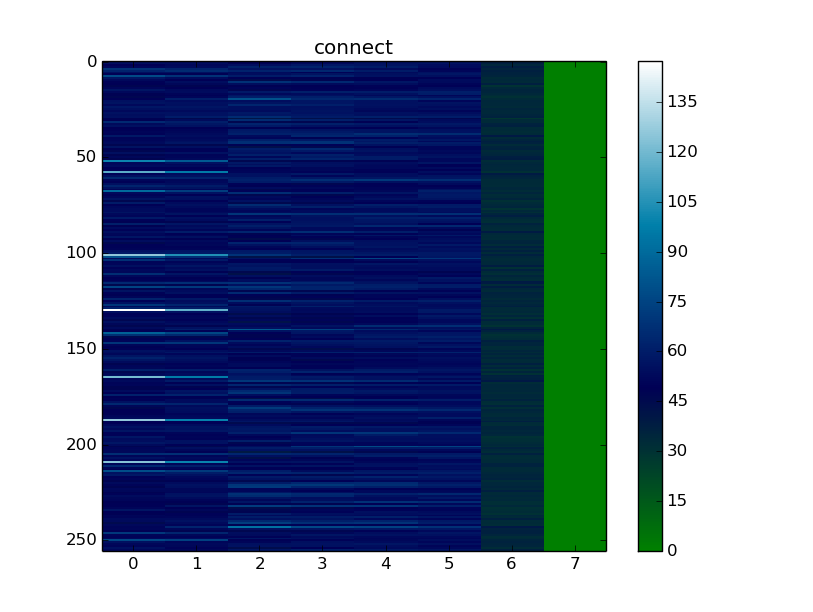
\includegraphics[scale=0.4]{pictures/1per300_tracefile_connect.png}
\caption{Visualized trace file}
\end{figure}
